%*****************************************
\chapter{Diferenciación}\label{ch:diferenciacion}
%*****************************************
\section{Límites y continuidad}

Esta sección está centrada en los conceptos de conjunto abierto, límite y continuidad; los conjuntos abiertos son necesarios para entender los límites y, a su vez, los límites son necesarios para entender continuidad y diferenciabilidad.

Comenzamos la formulación del concepto de conjunto abierto mediante la definición de disco abierto. Sea $x_{0}
\in  \realR^{n}$ y sea $r$ un número real positivo. El disco abierto (o bola abierta) de radio $r$ y centro 
en $x_{0}$, como vimos en el Ejemplo \ref{ex:distance}, es el conjunto de puntos $x$ tales que $\|x-x_{0}\| < r $.
Este conjunto lo denotaremos por $D_{r}(x_{0})$.

\begin{definition}
    Sea $U \subset \realR^{n}$. Decimos que $U$ es un conjunto abierto cuando para cualquier punto $x_{0}$ en $U$ existe algún $r>0$
    tal que $D_{r}(x_{0})$ está contenido en $U$, es decir, $D_{r}(x_{0}) \subset U$.
\end{definition}

\begin{figure}[!ht]
  \begin{center}
      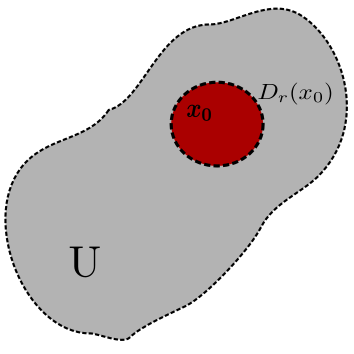
\includegraphics[width=0.5\linewidth]{gfx/conjunto-abierto}
      \caption{Un conjunto abierto $U$ es aquel que incluye completamente algún disco $D_{r}(x_{0})$ alrededor
      de cada uno de sus puntos $x_{0}$.}
      \label{fig:boat1}
  \end{center}
\end{figure}

Además establecemos la convención de que el conjunto vac/'io $\emptyset$ es abierto.

\begin{theorem}
    Para cada $x_{0} \in \realR^{n}$ y $r > 0$, $D_{r}(x_{0})$ es un conjunto abierto.
\end{theorem}

\begin{proof}
    Sea $x \in D_{r}(x_{0})$, esto es, sea $\|x - x_{0}\| < r$. De acuerdo con la definición
    de conjunto abierto, debemos encontrar un $s > 0$ tal que $D_{s}(x) \subset  D_{r}(x_{0})$.
    Sea $s = r - \|x - x_{0}\|$, nótese que $s > 0$, pero que $s$ se hace más chico si $x$ está
    cerca del borde $D_{r}(x_{0})$ \\

    Para probar que $D_{s}(x) \subset D_{r}(x_{0})$, sea $y \in D_{s}(x)$; esto es, sea
    $\|y - x\| < s$. Queremos probar que también $y \in D_{r}(x_{0})$. Probar esto en vista
    de la definición de un r-disco, equivale a demostrar que $\|y -x_{0}\| < r$. Usemos la desigualdad
    del triángulo para esto

    \begin{eqnarray*}
        \|y - x_{0}\| &=& \|(y - x) + (x - x_{0})\| \\
                              &\le& \|y - x\| + \|x - x_{0}\| \\
                              &<& s + \|x-x_{0}\| \\
                              &=& r \text{.}
    \end{eqnarray*}

    De aquí que $\|y - x_{0}\| < r$. \qed

\end{proof}

\begin{definition}
    Sea $A \subset \realR^{n}$. Un punto $x \in \realR^{n}$ es punto frontera de $A$ si toda vecindad de $x$ contiene al menos un punto de $A$ y al menos un punto fuera de $A$.
\end{definition}

En esta definición, $x$ puede estar o no en $A$; si $x \in A$, entonces $x$ es un punto frontera si toda vecindad de $x$ contiene al menos un punto
que no esté en $A$. De manera análoga, si $x$ no está en $A$, es un punto frontera si toda vecindad de
$x$ contiene al menos un punto de $A$.

\begin{figure}[!ht]
  \begin{center}
      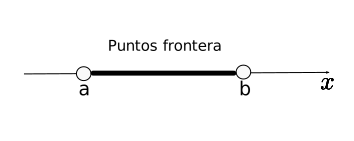
\includegraphics[width=0.5\linewidth]{gfx/puntos-frontera}
      \caption{}
      \label{fig:boat1}
  \end{center}
\end{figure}


Ya estamos en posición de definir un límite. Durante toda la exposición siguiente, el dominio de definición de la función $f$ será un conjunto abierto $A$.
Nos interesa encontrar el límite de $f$ cuando $x \in A$ tienda a un punto de $A$ o a un punto frontera de $A$.

El concepto de límite es una herramienta básica y útil para el análisis de funciones; nos permite estudiar derivadas y de especial interes en este texto,
derivadas parciales.

\begin{definition}[Límite]
    Sea $f:A \subset \realR^{n} \mapsto \realR^{m}$, donde $A$ es un conjunto abierto. Sea $x_{0}$ un punto de $A$ o en la frontera de $A$, y sea
    $V$ una vecindad de $\bm{b} \in \realR^{m}$. Decimos que $f$ está en $V$ conforme $x$ tiende a $x_{0}$ si existe una vecindad $U$ de 
    $x_{0}$ tal que $x \neq x_{0}$, $x \in U$ y $x \in A$ implica $f(x) \in V$. Decimos que $f(x)$ tiende a $\bm{b}$ cuando
    $x$ tiende a $x_{0}$, es decir

    $$ \lim_{x \rightarrow x_{0}} f(x) = b $$
\end{definition}

Del cálculo de una variable sabemos que el concepto de función continua está basado en la idea intuitiva de una función cuya gráfica es una
curva sin romper, esto es, una curva sin saltos.

\begin{definition}
    Sea $f:A \subset \realR^{n} \mapsto \realR^{m}$ una función dada con dominio $A$ y $x_{0} \in A$. Decimos que $f$ es continua
    en $x_{0}$ si
    $$ \lim_{x \rightarrow x_{0}} f(x) = f(x_{0})\text{.}$$
\end{definition}

Si decimos simplemente que $f$ es \emph{continua}, queremos decir que $f$ es continua
en cada punto $x_{0}$ de $A$.

\section{Diferenciación}

En nuestro trabajo de la sección anterior vimos qué es una función continua. Aquí veremos que significa que una función sea diferenciable y como
esto nos ayuda a ver que una gráfica no esté rota, es decir, no debe haber dobleces, esquinas o picos en la gráfica. En otras palabras, la gráfica 
debe ser suave.

Para precisar estas ideas necesitamos una definición sensata de lo que entedemos por $f(x_{1}, \ldots, x_{n})$ es diferenciable en $x=(x_{1}, \ldots, x_{n})$.
Para ello necesitamos introducir el concepto de \emph{derivada parcial}. Este concepto se
basa en nuestro conocimiento del cálculo en una variable.

Entonces comenzaremos con definir que significa que $f(x)$ es diferenciable en un punto $x$, es decir, la derivada de $f(x)$ en $x$. Para esto usaremos
nuestra definición de límite.

\begin{definition}
    Sea $f$ una función de valor real definida en una vecindad abierta de $x$. Entonces $\frac{df}{dx}$ (la derivada de $f$ respecto a $x$) es
    $$ \lim_{h \rightarrow 0} \frac{f(x+h) - f(x)}{h} $$
\end{definition}

En ocasiones usaremos la notación $f'(x)$ para denotar la derivada de $f$ respecto $x$.

\begin{example}
    Sea $f(x)=x^{2}$ ( figura \ref{fig:derivative} ), entonces
    \begin{eqnarray*}
        f'(1) &=& \lim_{h \rightarrow 0} \frac{f(1+h)-f(1)}{h} \\
              &=& \lim_{h \rightarrow 0} \frac{(1+h)^{2}-(1)}{h} \\
              &=& \lim_{h \rightarrow 0} (2 + h) \\
              &=& 2 \text{.}
    \end{eqnarray*}
    Entonces $f'(1) = 2$.
\end{example}

\begin{figure}[!ht]
  \begin{center}
      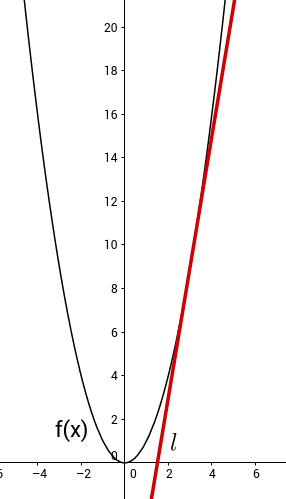
\includegraphics[width=0.5\linewidth]{gfx/derivative-example}
      \caption{$f(x)=x^{2}$}
      \label{fig:derivative}
  \end{center}
\end{figure}

De forma geométrica para una funci\'on $f:\realR \rightarrow \realR$, la derivada nos dice la \emph{pendiente} de la recta tangente a $f$ en un punto $x$.

Que una función $f(x)$ sea diferenciable en todo su dominio quiere decir que para cualquier $x$ en el dominio de $f(x)$ existe
$f'(x)$, esto nos dice que la gráfica de $f(x)$ es suave. Esto nos acerca a la definición de \emph{curva}. Un ejemplo típico 
de una gráfica no suave la vemos a continuci\'on:

\begin{example}
    Sea $f(x) = |x|$ ( figura \ref{fig:no-derivative} ) con $f:\realR \rightarrow \realR^{2}$, vemos que la derivada en $x=0$ no existe.
    \begin{eqnarray*}
        f'(0) &=& \lim_{h \rightarrow 0} \frac{f(h) - f(0)}{h} \\
              &=& \lim_{h \rightarrow 0} \frac{0}{0} \text{.}
    \end{eqnarray*}
\end{example}

\begin{figure}[!ht]
  \begin{center}
      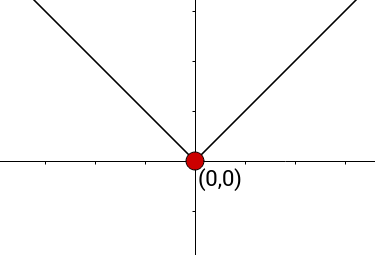
\includegraphics[width=0.55\textwidth]{gfx/grafica-abs}
      \caption{gráfica no suave}
      \label{fig:no-derivative}
  \end{center}
\end{figure}

Transportando esta idea a funciones de varias variables surge la definición de \emph{derivada parcial}.

\begin{definition}
    Sean $U \subset \realR^{n}$ un conjunto abierto y $f:U \subset \realR^{n} \rightarrow \realR$ una función con valores reales. Entonces $\partial f/\partial x_{1},
    \ldots, \partial f/ \partial x_{n}$, las derivadas parciales de $f$ respecto a la primera, segunda, \dots, n-ésima variable son las funciones con valores
    reales, de $n$ variables, las cuales, en el punto $(x_{1},\ldots,x_{n}) = x$, están definidas por
    \begin{eqnarray*}
        \frac{\partial f}{\partial x_{j}} (x_{1},\ldots,x_{n}) &=& \lim_{h \rightarrow 0} \frac{f(x_{1},x_{2},\ldots,x_{j} + h,\ldots,x_{n}) - f(x_{1},\ldots,x_{n})}{h} \\
                                                               &=& \lim_{h \rightarrow 0} \frac{f(x+he_{j})-f(x)}{h} 
    \end{eqnarray*}
    si existen los límites, donde $1 \le j \le n$ y $e_{j}$ es el j-ésimo vector de la base canónica.
\end{definition}

En otras palabras, $\partial f / \partial x_{j}$ es simplemente la derivada de $f$ respecto a la variable $x_{j}$, manteniendo las otras variables fijas.

\begin{myExample}
    Si $f(x,y) = x^{2}y+y^{3}$, encontrar $\partial f / \partial x$ y $\partial f / \partial y$.
    Para encontrar $\partial f / \partial x$ mantenemos $y$ constante y diferenciamos sólo respecto de $x$, entonces
    $$ \frac{\partial f}{\partial x} = \frac{d(x^{2}y+y^{3})}{dx} = 2xy \text{.} $$

    De forma análoga, tenemos que
    $$ \frac{\partial f}{\partial y} = \frac{d(x^{2}y+y^{3})}{dy} = x^{2} + 3y^{2} \text{.} $$
\end{myExample}
%*****************************************
%*****************************************
%*****************************************
%*****************************************
%*****************************************
